\documentclass{ensta_paris_pre_rapport} % Utilisation du modèle de rapport de l'ENSTA Paris
\def\enstaLogo{ensta.jpg} % Logo de l'école
\def\hostLogo{ensta.jpg} % Logo de l'entreprise ou de l'institut de recherche
\def\documentTitle{Projet de Recherche (PRe)} % Titre du document
\def\speciality{Informatique} % Spécialité
\def\academicYear{2023-2024} % Année académique
\def\title{Application de l'IA à l'analyse des données} % Titre du projet
\def\authorName{Jean Dupont} % Nom de l'auteur
\def\schoolTutor{Pierre Martin} % Nom du tuteur de l'école
\def\classPromotion{2026} % Promotion
\def\hostTutor{Lucie Lefevre} % Tuteur à l'entreprise ou à l'institut de recherche
\def\internshipDuration{Stage éffectué du 01/06/2023 au 31/08/2023} % Durée du stage
\def\hostName{Institut de Recherche en Informatique} % Nom de l'entreprise ou de l'institut de recherche
\def\hostAddress{123 rue de la Science, 75000 Paris - France} % Adresse de l'entreprise ou de l'institut de recherche
\setboolean{confidential}{true} % Confidentialité du rapport
\setboolean{onlinePublish}{true} % Publication en ligne autorisée


% Pied de page personnalisé
\fancyfoot[C]{
    \textit{\MyFooter}\par
    {\color{red}\textit{
        Rapport 
        \ifthenelse{\boolean{confidential}}{confidentiel}{non confidentiel et
        \ifthenelse{\boolean{onlinePublish}}{publiable}{non publiable}
        sur internet}}
        }
}
\rfoot{\thepage}
\begin{document}

% Inclusion des différentes sections du rapport

\begin{titlepage}
	\includegraphics[height=4cm]\enstaLogo
	\hfill
	\includegraphics[height=4cm]\hostLogo
	\par\vspace{0.5cm}
	\centering % Everything on this page will be centered
	    
	\vspace*{\fill} % Vertically center the page contents
	
	    
	\textbf{\Huge \documentTitle}\par\vspace{1.5cm}
	\textbf{\Large Spécialité : \speciality}\par\vspace{0.5cm}
	\textbf{\Large Année scolaire : \academicYear}\par\vspace{1.5cm}
	{\Huge\bfseries \title}\par\vspace{1cm}
	\vspace{1cm}
	\fcolorbox{red}{white}{\parbox{0.8\linewidth} {
		\centering
		\vspace{0.3cm}
		\color{red}\textbf{\Large Mention de confidentialité}\par
		\vspace{0.3cm}
		\textbf{ 
			\ifthenelse{\boolean{confidential}}{le document est confidentiel}{le document est non confidentie. \ifthenelse{\boolean{onlinePublish}}{Il peut donc être consultable en ligne par tous.}{et consultable au format électronique uniquement sur place à la bibliothèque de l'ENSTA Paris.}}
		}
		\vspace{0.3cm}
		}
	}
	    
	\vspace{1cm}
	\begin{multicols}{2}
		\textbf{\small Auteur :\authorName}\par
		\textbf{\small Tuteur ENSTA Paris : \schoolTutor}\par
		\columnbreak
		\textbf{\small Promotion: \classPromotion}\par
		\textbf{\small Tuteur organisme d'accueil : \hostTutor}\par
	\end{multicols}
	\par\vspace{1cm}
	\textbf{\large\internshipDuration}\par\vspace{1cm}
	{\raggedleft
		\textbf{NOM de l'organisme d'accueil : \hostName}\par
		\textbf{Adresse : \hostAddress}\par
	}
	    
	\vspace*{\fill} % Vertically center the page contents
\end{titlepage} % Page de titre
~\newpage
\section*{Résumé}
\addcontentsline{toc}{section}{Résumé}

\lipsum[3]

\vspace{0.3cm}
\textbf{Mots-clés: }keyword1, keyword2, keyword3

\vfill

\section*{Abstract}

\lipsum[4]

\vspace{0.3cm}
\textbf{Keywords: }keyword1, keyword2, keyword3

\vfill

\newpage % Résumé
~\newpage
\section*{Remerciements}
\addcontentsline{toc}{section}{Remerciements}
\lipsum[1]
\newpage
 % Remerciements

% Table des matières
\tableofcontents
\newpage

% Table des figures
\listoffigures
\newpage

\section{Section}
\lipsum[6]\cite{dupont2023}
\subsection{Subsection}
\lipsum[8] Voir Figure \ref{Fig1}.

\begin{figure}[h]
\centering
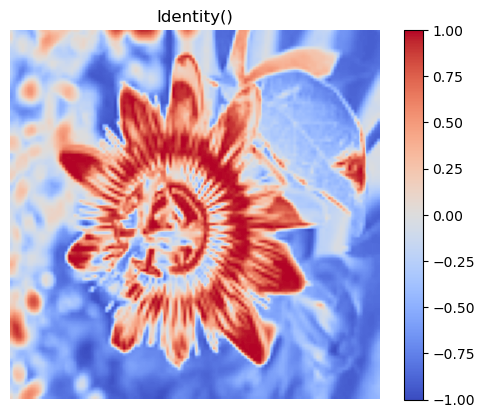
\includegraphics[width=0.7\textwidth]{figure1.png}
\caption{Exemple Figure}
\label{Fig1}
\end{figure}

\subsubsection{Subsubsection}
\lipsum[9] % Section 1

\newpage
\bibliographystyle{plain} % Style de la bibliographie
\bibliography{ref.bib} % Fichier de références bibliographiques
\addcontentsline{toc}{section}{Bibliographie}

\newpage
\appendix
\section{Annexes 1}
\lipsum[2]
\subsection{sub}
\lipsum[1] % Annexes

\end{document}
